\chapter{Introduction}
\label{sec:theory}

\section{The Standard Model of particle physics}

The Standard Model (SM) is a quantum field theory governing the kinematics and interactions of a set of fermion fields, respecting Lorentz and local gauge symmetries.
The SM gauge group $G$ decomposes into an electroweak sector (with symmetry group $\U(1) \times \SU(2)$)~\cite{weak1,weak2,weak3} and a strong sector ($\SU(3)$)~\cite{qcd1,qcd2}.
The action of $G$ on a fermion depends on the representation of the Lie group in which the fermion resides and the coupling strength.
For the special unitary groups, we denote the representation as $\mathbf{N}$ (fundamental), $\bar{\mathbf{N}}$ (anti-fundamental), or $\mathbf{1}$ (trivial).
The special unitary gauges have the same interaction strength for all fermions in non-trivial representations (known as universality).
All fermions are in a one-dimensional representation of $\U(1)$, but the weak hypercharge ($Y_W$) distinguishes their transformation under the gauge group $f\mapsto f + i Y_W g' f$, where $g'$ is the coupling strength of $\U(1)$.

Table~\ref{tab:theory:fermions} gives a summary of the \emph{first generation} SM fermion fields and the representation of $G$ which acts on them.
The SM provides a total of 3 generations of fermions, each of them copies of the first generation in terms of the field content and gauge group action.

\begin{table}[]
\begin{center}
    \caption{First generation SM fermions and the action of the SM local gauge symmetry group $G$.
             The subscripts $L$ and $R$ refer to left- and right-handed chirality fields.
             Not shown are the charge conjugated fields $f^C \equiv Cf$, which sit in conjugated representations.}
    \label{tab:theory:fermions}
    \begin{tabular}{l|c|c|c|c}
                Name & Symbol       & $Y_W$ & $\SU(2)$ rep. & $\SU(3)$ rep. \\
                \hline \hline
  Left-handed lepton & $\ell_L$     & $-\nicefrac{1}{2}$  & $\mathbf{2}$  & $\mathbf{1}$ \\  
 Right-handed charged lepton & $e_R^-$   & $-1$  & $\mathbf{1}$  & $\mathbf{1}$ \\  
 Right-handed neutrino & $\nu_R$   & $0$  & $\mathbf{1}$  & $\mathbf{1}$ \\  \hline
  Left-handed quark  & $q  _L$     & $\nicefrac{1}{6}$  & $\mathbf{2}$  & $\mathbf{3}$ \\  
 Right-handed up quark  & $u  _R$     & $\nicefrac{2}{3}$  & $\mathbf{1}$  & $\mathbf{3}$ \\ 
 Right-handed down quark  & $d  _R$     & $-\nicefrac{1}{3}$  & $\mathbf{1}$  & $\mathbf{3}$ \\  
    \end{tabular}
\end{center}
\end{table}

The lepton doublets contain the left-handed charged leptons and neutral neutrinos:
\begin{equation}
    \ell_{iL} = 
    \left(\begin{matrix} \nu_e \\ e_L^- \end{matrix}\right),
    \left(\begin{matrix} \nu_\mu \\ \mu_L^- \end{matrix}\right),
    \left(\begin{matrix} \nu_\tau \\ \tau_L^- \end{matrix}\right)
\end{equation}
where $i$ indexes the generation.
The right handed lepton singlets contain the right-handed projections of the same fermions.

The quark (electroweak) doublets contain the left-handed up- and down-type quarks:
\begin{equation}
    q_{iL} = 
    \left(\begin{matrix} u_L \\ d'_L \end{matrix}\right),
    \left(\begin{matrix} c_L \\ s'_L \end{matrix}\right),
    \left(\begin{matrix} t_L \\ b'_L \end{matrix}\right)
\end{equation}
where $d',s',b'$ represent linear combinations of the mass eigenstates $d,s,b$ (discussed further in Section~\ref{sec:theory:ewk}).
All quarks also sit in a strong triplet; we have suppressed its charge above, as the strong representation is orthogonal to the electroweak representation.
Where necessary, it will be specified with a superscript, i.e. $u^{c}$.

\subsection{Quantum chromodynamics}
The dynamics of quarks under the $\SU(3)$ gauge group is commonly referred to as the strong interaction or quantum chromodynamics (QCD).
The QCD Lagrangian is:
\begin{equation}
    \mathcal{L}_\mathrm{QCD} = 
        i \bar q^{a}_f \slashed D^{ab} q^{b}_f  
        + m_f \bar{q}^{a}_f q^{a}_f
        - \frac{1}{4} G^{a}_{\mu\nu} G^{a,\mu\nu}
    \label{eq:theory:lqcd}
\end{equation}
where repeated indices are contracted; $q_f=u,d,c,s,b,t$ are the spinors for each quark flavor $f$; $a,b=r,g,b$ are the colors (basis elements of the triplet representation); $m_q$ is the mass of quark flavor $q$.
$D_\mu$ is the QCD covariant derivative:
\begin{equation}
    D_\mu^{ab} = \delta^{ab} \partial_\mu - i g_s \sum_c t^{ab}_c G_{c,\mu}
\end{equation}
where $g_s$ is the strong coupling strength; $t_c$ are the 8 generators of the triplet representation of $\SU(3)$; $G_c$ are the corresponding 8 gauge boson (gluon) fields. 
$G^a_{\mu\nu}$ are the gluon field strength tensors:
\begin{equation}
    G^a_{\mu\nu} = \partial_\mu G_\nu^a - \partial_\nu G_\mu^a - g_s f^{abc} G_\mu^b G_\nu^c
\end{equation}
where $f^{abc}$ are the structure constants of $\SU(3)$.

An additional term can be added to Equation~\ref{eq:theory:lqcd} without violating any guage or Lorentz symmetry or renormalizability.
This term would violate CP conservation and produce a non-zero electric dipole moment (EDM) for the neutron.
Experimental constraints on the neutron EDM (e.g. Reference~\cite{nedm1}) place strong upper limits on this CP violation, and so we do not consider it as part of the SM QCD Lagrangian. 

\subsubsection{Renormalization and running of couplings}

Physical quantities in a QFT (couplings, masses, field strengths, operators) acquire a scale-dependence from higher-order corrections to vertices and propagators. 
In many cases, the quantum corrections to the bare parameter contain ultraviolet divergent terms.
These infinities are absorbed into the Lagrangian by means of adding so-called counterterms. 
The systematic process of absorbing these infinities and ensuring scale-independence is known as renormalization.
A Lagrangian is called \emph{renormalizable} if only a finite number of counterterms are needed to ensure that all observables (i.e. amplitudes) are finite. 
The SM is a renormalizable theory.

In this discussion, we will focus on the renormalization of the coupling $\alpha_S \equiv \nicefrac{g_s^2}{4\pi}$, but the argument applies broadly to all SM quantities.
There are two related consequences of quantum corrections: $\alpha_S$ acquires a non-trivial dependence on the energy scale at which it is probed ($\mu_R^2 = -q^2$, where $q^\mu$ is the gluon momentum); and the \emph{bare} $\alpha_S$ as written in the Lagrangian is not the same as the $\alpha_S(\mu_R^2)$ measured in the laboratory.
We will refer to the bare coupling as $\alpha_{S0}$. 
Note that it does not have a $\mu_R^2$-dependence.
To enforce this, we look for solutions to the differential equation
\begin{equation}
    \mu_R^2 \frac{\di \alpha_{S0}}{\di\mu_R^2} = 0
\end{equation}
Writing $\alpha_{S0}$ in terms of $\alpha_S$ (which has a $\mu_R^2$-dependence) and rearranging the terms, we arrive at the \emph{$\beta$ function} for $\alpha_S$:
\begin{equation}
    \beta(\alpha_S) \equiv \mu_R^2 \frac{\di \alpha_S}{\di\mu_R^2} = -\left(\beta_0 \alpha_S^2 + \beta_1 \alpha_S^3 + \mathcal{O}(\alpha_S^4)\right)
\end{equation}
The $\beta$ coefficients are:
\begin{align}
    \beta_0 = \frac{33 - 2n_{f}}{3},~ 
    \beta_1 = \frac{153-19n_f}{24\pi^2} ,\dots
\end{align}
where $n_f$ is the number of quark flavors with masses below $\mu_R$~\cite{pdg,qcd1,qcd2}.
To one-loop order, the solution to this differential equation is:
\begin{equation}
    \alpha_S(\mu_R) = \frac{2\pi}{\beta_0 \ln \frac{\mu_R}{\Lambda_\mathrm{QCD}}}
\end{equation}
where $\Lambda_\mathrm{QCD}$ is set by enforcing a measured boundary condition, e.g. $\alpha_S(m_Z^2) = 0.1181 \pm 0.0011$~\cite{pdg}.
The exact value of $\Lambda_\mathrm{QCD}$ depends on the number of flavors ($n_f=5$ at $m_Z$) and the renormalization scheme (most commonly used is $\overline{\text{MS}}$~\cite{msbar}); with these conditions, $\Lambda_\mathrm{QCD} = 218$ MeV.
$\beta_0>0$ implies $\alpha_S$ falls as a function of energy, as illustrated in Figure~\ref{fig:theory:alphas}.

This running (the opposite of theories like quantum electrodynamics, in which $\beta_0<0$) results in an asymptotically ($\mu_R\rightarrow \infty$) free theory.
Below $\Lambda_\mathrm{QCD}$, the coupling constant is larger than order unity and perturbative QCD (pQCD) cannot make predictions in this regime.
This long-range behavior also means that color triplet (quarks, antiquarks) or octet (gluons) states cannot be observed. 
Only composite singlet states (hadrons) are observable. 

\begin{figure}[]
\begin{center}
    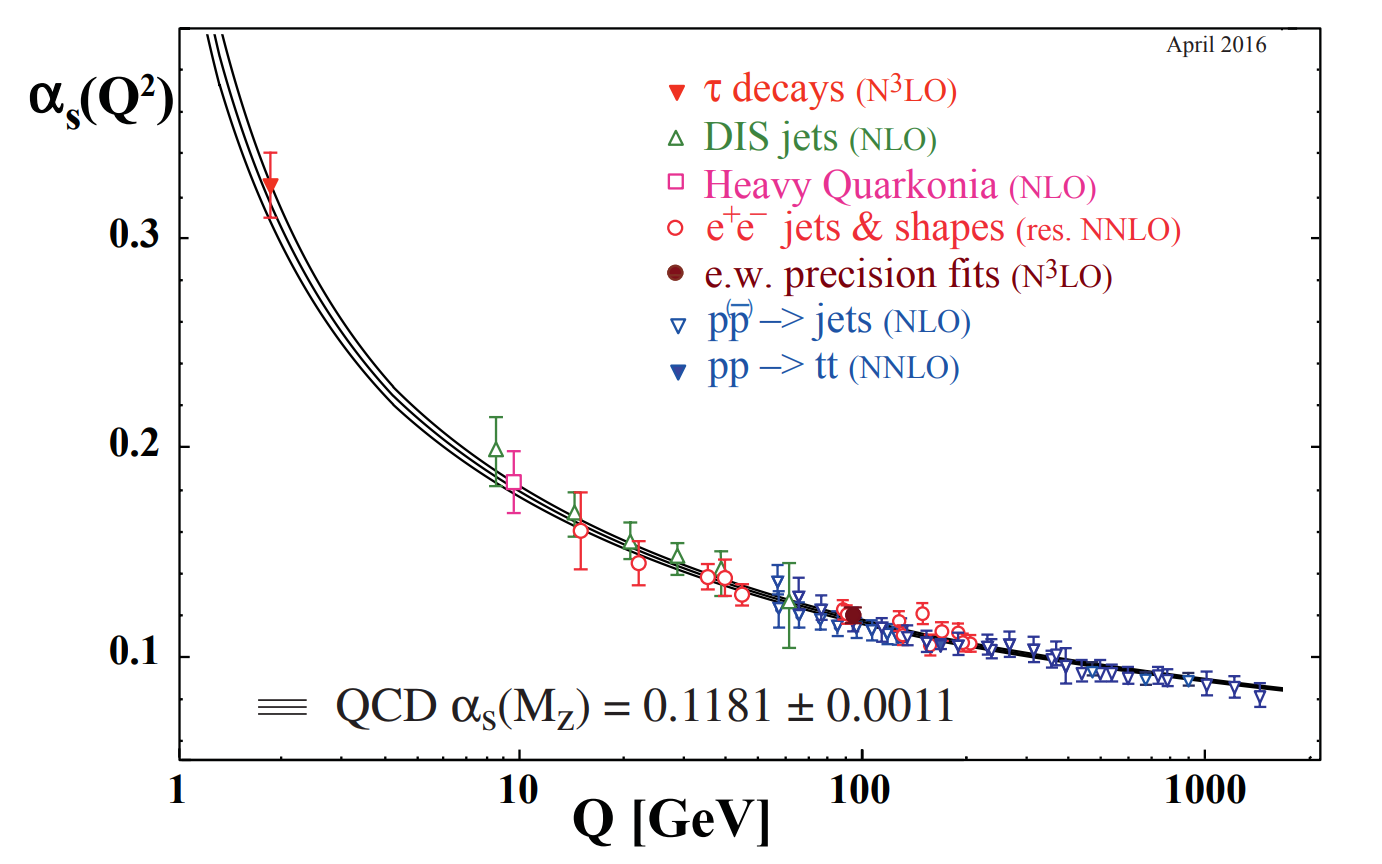
\includegraphics[width=0.6\textwidth]{figures/theory/alphas.png}
    \caption{Running of the QCD coupling strength $\alpha_S$ as a function of length scale.
             Reprinted from Reference~\cite{pdg}.}
    \label{fig:theory:alphas}.
\end{center}
\end{figure}

\subsection{Electroweak interactions}
\label{sec:theory:ewk}
The electroweak (EW) sector of the SM refers to the $\SU(2)\times\U(1)$ symmetry group.
While all fermion fields in Table~\ref{tab:theory:fermions} transform under $\U(1)$, only left-handed fermions have non-trivial transformations under $\SU(2)$.
The EW Lagrangian (ignoring particle masses and the Higgs sector for now) is:
\begin{align}
\mathcal{L}_\mathrm{EW} =~
        & i\bar\ell_{iL} \left(\slashed\partial-ig \slashed W^a \tau^a - ig'Y_{\ell_L} \slashed B\right)\ell_{iL} 
      + i\bar q_{iL}^{c} \left(\slashed\partial-ig \slashed W^a \tau^a - ig'Y_{q_L} \slashed B\right)q_{iL}^{c} \nonumber \\
      & + i\bar e_{iR} \left(\slashed\partial-ig'Y_{ e_R}\slashed B\right) e_{iR} 
       + i\bar u_{iR^{c}} \left(\slashed\partial-ig'Y_{u_R}\slashed B\right) u_{iR}^{c} 
       + i\bar d_{iR}^{c} \left(\slashed\partial-ig'Y_{d_R}\slashed B\right) d_{iR}^{c} \nonumber \\ 
      & - \frac{1}{4} W_{\mu\nu}^a W^{a,\mu\nu} - \frac{1}{4} B_{\mu\nu} B^{\mu\nu}  
      \label{eq:theory:lew}
\end{align}
where repeated indices are contracted; the subscript $i$ indexes generations; $g$ and $g'$ are respectively the coupling strengths for $\SU(2)$ and $\U(1)$; $Y$ is the weak hypercharge; $W_\mu^a$ are the three gauge fields corresponding to the generators $\tau^a = \nicefrac{\sigma^a}{2}$ of $\SU(3)$; $B_\mu$ is the gauge field for $\U(1)$; and $W_{\mu\nu}^a$ and $B_{\mu\nu}$ are the field strength tensors for the respective gauge fields.
The covariant derivative can be written as:
\begin{equation}
    D_\mu = \partial_\mu - ig\delta_L W^a_\mu \tau^a - ig' YB_\mu
\end{equation}
where $Y$ is the particle's hypercharge and $\delta_L$ is 1 if the field is in the $\mathbf{2}$ representation of $\SU(2)$ (e.g. left-handed fermions) and 0 otherwise. 

\subsubsection{EW symmetry breaking}
Unlike Equation~\ref{eq:theory:lqcd}, we cannot introduce a quadratic mass term for fermions in Equation~\ref{eq:theory:lew} because $\bar\psi \psi = \psi^\dag_R\psi_L + \psi^\dag_L\psi_R$ is not invariant under $\SU(2)$ rotations.
Spontaneous electroweak symmetry breaking remedies this, as well as provides masses for the gauge fields~\cite{ewsb1,ewsb2,ewsb3,ewsb4,ewsb5,ewsb6}.
A complex scalar doublet $\phi$ (called the complex Higgs field) with $Y_\phi=\nicefrac{1}{2},~\delta_L=1$ is added to the Lagrangian:
\begin{equation}
    \mathcal{L}_\mathrm{EW} \mapsto \mathcal{L}_\mathrm{EW}
            + |D_\mu \phi|^2 + \mu^2|\phi|^2 - \lambda |\phi|^4
    \label{eq:theory:lhiggs}
\end{equation}
We can write the complex doublet as 4 real fields:
\begin{equation}
    \phi = \frac{1}{\sqrt{2}} \left(\begin{matrix} \phi_1 + i\phi_2 \\ \phi_3 + i \phi_4 \end{matrix} \right)
\end{equation}
The two self-interaction terms create a Higgs potential with a degenerate global minimum at \emph{vacuum expectation value} $v \equiv \langle |\phi| \rangle = \sqrt{\nicefrac{\mu^2}{\lambda}}$.
Through gauge rotations, we can fix $\langle\phi_{1,2,4}\rangle = 0$ and, at low energies, expand $\phi_3 = v + H$, where $H$ is the real Higgs field. 
This is the spontaneoous breaking of a symmetry.

By the Nambu-Goldstone theorem~\cite{nambu,goldstone}, these three lost degrees of freedom give rise to three massless bosons. 
The $|D_\mu \phi|$ term couples the complex Higgs field to the gauge bosons:
\begin{align}
    |D_\mu \phi|^2_{\phi = \langle\phi\rangle} &= 
        \frac{v^2}{8} \left[(gW_\mu^1)^2 + (gW^2_\mu)^2 + (g'B_\mu - gW_\mu^3)^2\right] 
\end{align}
The diagonization of this mass term gives 3 massive weak bosons (consuming the 3 massless Nambu-Goldstone bosons) and one massless photon (defining $\tan\theta_w = g'/g$):
\begin{align}
    W^\pm_\mu &\equiv \frac{W_\mu^1 \mp iW_\mu^2}{\sqrt{2}} \nonumber \\ 
    Z_\mu &\equiv \cos\theta_w W_\mu^3 - \sin\theta_w B_\mu \nonumber \\ 
    A_\mu &\equiv \sin\theta_w W_\mu^3 + \cos\theta_w B_\mu
\end{align}
with mass eigenvalues:
\begin{equation}
    m_W = \frac{gv}{2}, \quad m_Z = \frac{v\sqrt{g^2+g'^2}}{2}, \quad m_A = 0
\end{equation}

The remaining $H$ field, which has not been consumed, is the Higgs boson discovered by CMS and ATLAS~\cite{higgsdisc} in 2012.
It has mass $m_H = \sqrt2\mu$.
By expanding $\phi$ around $\langle \phi \rangle$ in Equation~\ref{eq:theory:lhiggs}, we find couplings to the massive gauge bosons:
\begin{gather}
    \frac{m_Z^2}{v} hZ_\mu Z^\mu, \quad \frac{2m_W^2}{v}hW^{+\mu} W^{-}_\mu, \nonumber \\
    \frac{m_Z^2}{2v} h^2 Z_\mu Z^\mu, \quad \frac{m_W^2}{v} h^2 W^{+\mu} W^-_\mu 
\end{gather}
The breaking of the $\SU(2)\times \U(1)$ symmetry leaves behind a local $\U(1)$ symmetry (with gauge boson $A_\mu$), which corresponds to electromagnetism.
Fermions have charge $eQ = e(T_3+Y)$, where $e=g'\cos\theta_w$ and $T_3$ is the third isospin component. 
The $W^\pm$ bosons receive charge $\pm e$.
After symmetry breaking, the actions of the broken gauge groups on fermions are governed by the following Lagrangian terms:
\begin{align}
    \La_\mathrm{EWSB} \supset 
            \sum_f &\left[\bar f\left(i\slashed\partial-eQ_f\slashed A\right) f 
            - \frac{g}{2\sqrt{2}} \bar f_L \left(T^+\slashed W^+ + T^- \slashed W^-\right) f_L\right. \nonumber \\
            &\left.~- \frac{g}{2\cos\theta_w} \bar f\left(g_{Vf} - g_{Af} \right)\slashed Z f \right]
\end{align}
where $f$ are all fermion fields; $f_L = \frac{1}{2}(1-\gamma^5)f$; $g_{V} = T_3- 2Q\sin^2\theta_w$; and $g_{A} = T_3$.

\subsubsection{Fermion masses}
The last piece of the EW Lagrangian is the addition of the fermion masses through Yukawa couplings with the Higgs doublet. 
First, let us add the terms for quark couplings:
\begin{equation}
   \La_\mathrm{EW} \mapsto \La_\mathrm{EW} - y_{ij}^d \bar q_{iL} \phi d_{jR} - y_{ij}^u \bar q_{iL}i\sigma_2 \phi^* u_{uR}i + \hc
\end{equation}
where $\hc$ refers to the Hermetian conjugate of preceding terms; and $y_{ij}^{u,d}$ are the Yukawa matrices for up- and down-type quarks.
Breaking the symmetry and collecting terms proportional to $v$:
\begin{equation}
    -\frac{v}{\sqrt{2}}\left(y_{ij}^d \bar d_{iL}' d_{jR} + y_{ij}^u \bar u_{iL} u_{jR}\right) 
\end{equation}
The mass eigenstates are found by diagonalizing these terms, which are written in terms of the weak eigenstates.
Let us denote the unitary transformations from the mass basis to the weak basis as $U_u$ and $U_d$. 
If we try to write the rest of $\La_\mathrm{EWSB}$ in terms of mass eigenstates, we see that terms of the following form all have trivial transformations:
\begin{gather} 
\bar d' \gamma^\mu d' \mapsto \bar d U_d^\dag \gamma^\mu U_d d = \bar d \gamma^\mu d
\end{gather}
The only non-trivial transformation is in the charged weak interaction:
\begin{align} 
\bar u_L \slashed W^+ d'_L + \bar d'_L W^- u_L &\mapsto 
    \bar u_L \slashed W^+ U_u^\dag U_d d_L + \bar d_L W^- U_d^\dag U_u u_L \nonumber \\
    &\equiv \bar u_L \slashed W^+ V_\mathrm{CKM} d_L + \bar d_L W^- V^\dag_\mathrm{CKM} u_L
\end{align}
where $V_\mathrm{CKM}$ is the Cabibbo-Kobayshi-Maskawa matrix~\cite{ckm1,ckm2}.
It is nearly-diagonal, but with non-zero mixing between the generations. 
The CKM matrix also contains a charge parity (CP) violating phase.
When referring to down-type quarks, we typically refer to the mass eigenstate $d$ as opposed to $d'$.

A similar analysis can be carried out for the lepton sector:
\begin{equation}
   \La_\mathrm{EW} \mapsto \La_\mathrm{EW} - y_{ij}^e \bar \ell_{iL} \phi e_{jR} - y_{ij}^\nu \bar \ell_{iL}i\sigma_2 \phi^* \nu_{uR}i + \hc
\end{equation}
The mixing matrix for leptons is the Pontecorvo-Maki-Nakagawa-Sakata matrix $U_\mathrm{PMNS}$~\cite{pmns}, which relates the weak eigenstates $\nu_e, \nu_\mu,\nu_\tau$ with the mass eigenstates $\nu_1,\nu_2,\nu_3$.
The values of the neutrino masses are known to be non-zero from the observation of neutrino oscillations~\cite{nuosc}.

After EWSB, each fermion mass eigenstate has a mass term and coupling to the Higgs field:
\begin{equation}
    -\frac{y_f v}{\sqrt{2}} \left( \bar ff + \bar fH f\right)
\end{equation}
where we identify the mass as $m_f = y_f v/\sqrt{2}$. 
Table~\ref{tab:theory:ewsb} summarizes all SM fermions and some of their properties after EWSB.

\begin{table}[]
\begin{center}
    \caption{Summary of the SM fields after electroweak symmery breaking.
             All masses are taken from the global fits compiled by the Particle Data Group~\cite{pdg}.}
    \label{tab:theory:ewsb}
    \begin{tabular}{l|c|c|c|c}
        Name & Symbol & Spin & Mass & $Q_e$  \\  \hline \hline
        gluon & $g^{ab}$ & 1 & 0 & 0 \\   
        photon & $\gamma $ & 1 & 0 & 0 \\   
        $Z$ boson & $Z$ & 1 & 91.2 GeV & 0 \\   
        $W$ boson & $W^{\pm}$ & 1 & 80.4 GeV & $\pm 1$ \\   \hline 
        Higgs boson & $H$ & 0 & 125 GeV & $0$ \\   \hline 
        up quark & $u$ & $\nicefrac{1}{2}$ & $2.2$ MeV & $\nicefrac{2}{3}$    \\   
        down quark & $d$  & $\nicefrac{1}{2}$ & $4.7$ MeV  & $-\nicefrac{1}{3}$  \\   
        charm quark & $c$  & $\nicefrac{1}{2}$ & $1.28$ GeV  & $\nicefrac{2}{3}$  \\   
        strange quark & $s$  & $\nicefrac{1}{2}$ & $95$ MeV  & $-\nicefrac{1}{3}$  \\   
        top quark & $t$  & $\nicefrac{1}{2}$ & $173$ GeV  & $\nicefrac{2}{3}$  \\  \hline
        bottom quark & $b$  & $\nicefrac{1}{2}$ & $4.18$ GeV  & $-\nicefrac{1}{3}$  \\   
        electron neutrino  & $\nu_e$  & $\nicefrac{1}{2}$ & $-$  & $0$  \\   
        electron  & $e$  & $\nicefrac{1}{2}$ & $511$ keV  & $-1$  \\   
        muon neutrino  & $\nu_\mu$  & $\nicefrac{1}{2}$ & $-$  & $0$  \\   
        muon  & $\mu$  & $\nicefrac{1}{2}$ & $105$ MeV  & $-1$  \\   
        tau neutrino  & $\nu_\tau$  & $\nicefrac{1}{2}$ & $-$  & $0$  \\ 
        tau  & $\tau$  & $\nicefrac{1}{2}$ & $178$ GeV  & $-1$  \\   
    \end{tabular}
\end{center}
\end{table}

\section{LHC phenomenology}

The Large Hadron Collider collides protons at a center of mass energy $\sqrt{s} = 13$ TeV.
Section~\ref{sec:cms:lhc} provides an overview of the LHC machine.
In this section, we describe the methods used to make predictions of observables at the LHC.
These observables typically take the form of differential cross sections $\di\sigma(pp\rightarrow X)/\di\Theta$, where $X$ is some interesting final state with $N$ particles and $\Theta$ is a set of interesting kinematics.
The differential element of the general cross section for $2\rightarrow N$ processes is:
\begin{equation}
d\sigma(ab\rightarrow \{c_i\}) = 
    \frac{1}{2s} \left(\prod_i \dfrac{\mathrm{d}^3p_i}{(2\pi)^3} \frac{1}{2E_i}\right) 
        \cdot (2\pi)^4 \delta^4\left(k_a + k_b - \sum_i p_i\right) 
        \cdot \left|\Ma(ab\rightarrow \{c_i\})\right|^2
        \label{eq:theory:2n}
\end{equation}
where $k_a,k_b$ are the incoming momenta; $\{p_i\}$ are the outgoing momenta; and $\Ma$ is the matrix element of this reaction.
Hadron collisions do not have two-particle initial states, but rather two composite particles containing partons with varying momenta. 

The general cross section for $pp\rightarrow X$ is:
\begin{equation}
\di\sigma(pp\rightarrow X(\Theta)) = 
    \sum_{a,b} \int \mathrm{d}x_a \mathrm{d}x_b 
    ~f_a(x_a) f_b(x_b) 
    \cdot \di\sigma(ab\rightarrow\{c_i\}) 
    \cdot D(\{c_i\}\rightarrow X(\Theta))
    \label{eq:theory:master}
\end{equation}
The sum over $a,b$ refers to summing over partons in the initial state.
The momentum fractions of the partons, $x_{a,b}$, follow parton distribution functions (PDFs) $f_{a,b}$ that depend on the particle species $a$ and $b$. 
Any bare quark or gluon that is produced must form hadron(s) due to color confinement.
This process of \emph{hadronization} is not described by pQCD.
However, the production of most interesting final states at the LHC can be perturbatively analyzed.
Therefore, we split the process $ab\rightarrow X$ into $ab\rightarrow \{c_i\} \rightarrow X$.
The matrix element for the first step (\emph{hard scattering}) can usually be computed perturbatively and turned into a cross section by means of Equation~\ref{eq:theory:master}.
Other heuristic methods are used to deal with the second step (\emph{parton shower}), encoded in the \emph{fragmentation function} $D$. 

The ability to partition the calculation into perturbative (hard scattering) and non-perturbative (PDF and parton shower) components follows from the collinear factorization theorem~\cite{fact}.
The factorization depends on an arbitrary energy scale $\mu_F$, which defines a lower bound for radiation considered part of the hard scattering. 
The remainder of this section discusses the computation of these three factors: $f$, $\Ma$, and $D$.
